\documentclass[12pt, twoside]{article}
\usepackage[letterpaper, margin=1in, headsep=0.2in]{geometry}
\setlength{\headheight}{0.6in}
%\usepackage[english]{babel}
\usepackage[utf8]{inputenc}
\usepackage{microtype}
\usepackage{amsmath}
\usepackage{amssymb}
%\usepackage{amsfonts}
\usepackage{siunitx} %units in math. eg 20\milli\meter
\usepackage{yhmath} % for arcs, overparenth command
\usepackage{tikz} %graphics
\usetikzlibrary{quotes, angles}
\usepackage{graphicx} %consider setting \graphicspath{{images/}}
\usepackage{parskip} %no paragraph indent
\usepackage{enumitem}
\usepackage{multicol}
\usepackage{venndiagram}

\usepackage{fancyhdr}
\pagestyle{fancy}
\fancyhf{}
\renewcommand{\headrulewidth}{0pt} % disable the underline of the header
\raggedbottom
\hfuzz=2mm %suppresses overfull box warnings

\usepackage{hyperref}

\fancyhead[LE]{\thepage}
\fancyhead[RO]{\thepage \\ Name: \hspace{4cm} \,\\}
\fancyhead[LO]{BECA / Dr. Huson / Geometry\\*  Unit 1: Segments, length, and area\\* 16 Sept 2022}

\begin{document}

\subsubsection*{1.7 Exit Note Quiz: Length and perimeter, geometric notation}
\begin{enumerate}
  \item Various objects are depicted. Circle True or False for each statement.
  \begin{multicols}{2}
    \begin{tikzpicture}[scale=0.9]
      \draw[thick](0,0) node[above right]{$\ q$} --(6,0)--(8,4)--(2,4)--(0,0);
      \draw[<->, thick] (1,1)--(6,3);
      \draw[fill] (3.5,2) circle [radius=0.07] node[below=7pt]{$B \ $};
      \draw[fill] (5,2.6) circle [radius=0.07] node[below]{$D$};
      \draw[<->, thick] (2,3.5)--(5.25,.25);
      \draw[fill] (2.5,3) circle [radius=0.07] node[above right]{$A$};
      \draw[fill] (5,0.5) circle [radius=0.07] node[above right]{$C$};
    \end{tikzpicture}
    \begin{enumerate}
      \item T \quad F \quad The intersection of the two lines is point $D$.
      \item T \quad F \quad The line $\overleftrightarrow{AD}$ is shown.
      \item T \quad F \quad The plane is labeled $q$.
      \item T \quad F \quad $\overrightarrow{BA}$, $\overrightarrow{BC}$ are opposite rays.
    \end{enumerate}
  \end{multicols} \bigskip
  
\item Use symbols to write the name of each geometric figure.
\begin{enumerate}
  \begin{multicols}{3}
  \item \hspace{1cm}
    \begin{tikzpicture}[rotate=50]
      \draw[<->, thick] (1,0)--(1,3);
      \draw[fill] (1,0.5) circle [radius=0.05] node[above right]{$E$};
      \draw[fill] (1,2.5) circle [radius=0.05] node[below left]{$D$};
      \end{tikzpicture}
  \item
    \begin{tikzpicture}[rotate=-80]
      \draw[thick] (1,0)--(0,2);
      \draw[fill] (1,0) circle [radius=0.05] node[below]{$F$};
      \draw[fill] (0,2) circle [radius=0.05] node[below]{$G$};
      \end{tikzpicture}
  \item
    \begin{tikzpicture}[rotate=0]
      \draw[->, thick] (0,0)--(-3,1.5);
      \draw[fill] (0,0) circle [radius=0.05] node[below]{$K$};
      \draw[fill] (-2,1) circle [radius=0.05] node[below]{$J$};
      \end{tikzpicture}
  \end{multicols}
  \end{enumerate} \vspace{1cm}

\item Points in the same line are $\rule{4cm}{0.15mm}$. \bigskip

\item The line segment $\overline{TUV}$ is diagrammed below. 
  \begin{enumerate}
  \item Measure and label the lengths $TU$ and $UV$ to the nearest centimeter. \par  \bigskip
    \begin{tikzpicture}
      \draw[thick] (0,0)--(10,0);
      \draw[fill] (0,0) circle [radius=0.05] node[below]{$T$};
      \draw[fill] (3,0) circle [radius=0.05] node[below]{$U$};
      \draw[fill] (10,0) circle [radius=0.05] node[below]{$V$};
    \end{tikzpicture} \medskip
    \item Write an equation employing the Segment Addition Postulate.\par (fill in the blanks with values in centimeters) \par \bigskip
    $TV=$ \rule{2cm}{0.15mm} $+$ \rule{2cm}{0.15mm} $=$ \rule{2cm}{0.15mm}
  \end{enumerate} \medskip 

\item Points $R(7)$ and $S(32)$ are shown below. Find ${RS}$. \par \smallskip
  \begin{tikzpicture}[scale=0.25]
    \draw[<->] (-12,0)--(42,0);
    \foreach \x in {-10, -5,...,40}
      \draw[shift={(\x,0)}] (0pt,-16pt)--(0pt,16pt)node[below=5pt]{$\x$};
    \draw[fill] (7,0) circle [radius=0.2] node[above]{$R(7)$};
    \draw[fill] (32,0) circle [radius=0.2] node[above]{$S(32)$};
  \end{tikzpicture} \vspace{2cm}

\newpage
\item Given isosceles $\triangle XYZ$ with $\overline{XY} \cong \overline{XZ}$. On the diagram mark the congruent line segments with tick marks.
  \begin{center}
  \begin{tikzpicture}[scale=0.8]
    \draw[thick] (0,0)node[below]{$X$}--
      (4,0) node[below]{$Y$}--
      (58:4) node[above]{$Z$}--cycle;
  \end{tikzpicture}
  \end{center} \bigskip

\item Rectangle $ABCD$ is shown with length 10 centimeters and width 4 cm. Fill in the blanks and find the rectangle's perimeter.
  \begin{multicols}{2}
    \begin{flushleft}
    \begin{tikzpicture}[scale=0.7]
      \draw[thick]
        (0,0)node[below left]{$A$}--
        (6,0)node[below right]{$B$}--
        (6,3)node[above right]{$C$}--
        (0,3)node[above left]{$D$}--cycle;
      \node at (3,-0.8){$10$ cm};
      \node at (7,2){$4$ cm};
      \draw (2.9, -0.2)--(2.9,0.2);
      \draw (2.9, 2.8)--(2.9,3.2);
      \draw (-0.2, 1.4)--(0.2, 1.4);
      \draw (-0.2, 1.6)--(0.2, 1.6);
      \draw (5.8, 1.4)--(6.2, 1.4);
      \draw (5.8, 1.6)--(6.2, 1.6);
      \end{tikzpicture}
    \end{flushleft} 
  $P = 10 + 4 + \rule{1.5cm}{0.15mm} + \rule{1.5cm}{0.15mm} = \rule{1.5cm}{0.15mm}$
\end{multicols}

\item Given $\overline{PMQ}$, $M$ bisects $\overline{PQ}$, $PM=7x-12$, $MQ=3x$. Find ${PQ}$. (show check) \par \medskip
  \begin{flushleft}
    \begin{tikzpicture}
      \draw[thick] (0,0)--(6,0);
      \draw[fill] (0,0) circle [radius=0.05] node[below]{$P$};
      \draw[fill] (3,0) circle [radius=0.05] node[below]{$M$};
      \draw[fill] (6,0) circle [radius=0.05] node[below]{$Q$};
      \node at (1.5,0.7){$7x-12$};
      \node at (4.5,0.7){$3x$};
      \draw (1.4,-0.2)--(1.5,0.2);
      \draw (1.5,-0.2)--(1.6,0.2);
      \draw (4.4,-0.2)--(4.5,0.2);
      \draw (4.5,-0.2)--(4.6,0.2);
    \end{tikzpicture}
  \end{flushleft} \vspace{6cm}

  \item How do you think you did?

\end{enumerate}
\end{document}